\subsection{Colour Tests} % (fold)
\label{sub:colour_tests}
Depending on which house the user belongs to, the system should theme itself in that house's colours. The colour mappings are as follows:

\begin{table}[!htbp]
\centering
\begin{tabular}{|l|l|}
\hline
\multicolumn{1}{|c|}{\textbf{House}} & \multicolumn{1}{c|}{\textbf{Colour}} \\ \hline
Acton                                & Blue                                  \\ \hline
Baxter                               & Orange                               \\ \hline
Clive                                & Turquoise                            \\ \hline
Darwin                               & Purple                               \\ \hline
Houseman                             & Red                                  \\ \hline
Webb                                 & Yellow                               \\ \hline
\end{tabular}
\caption{House colours}
\end{table}

Screenshots showing that each house does produce the correct colours are below.
\clearpage

\begin{figure}[!htbp]
  \centering
  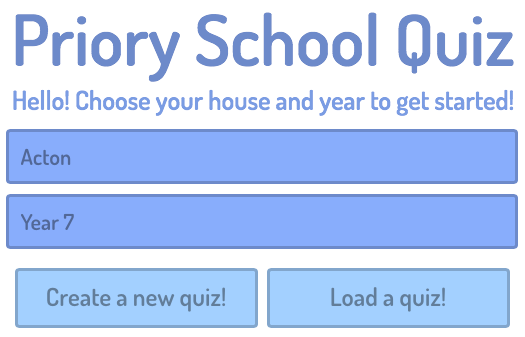
\includegraphics[scale=0.35]{testing/colours/acton}
  \caption{Test outcome for Acton's colours.}
\end{figure}

\begin{figure}[!htbp]
  \centering
  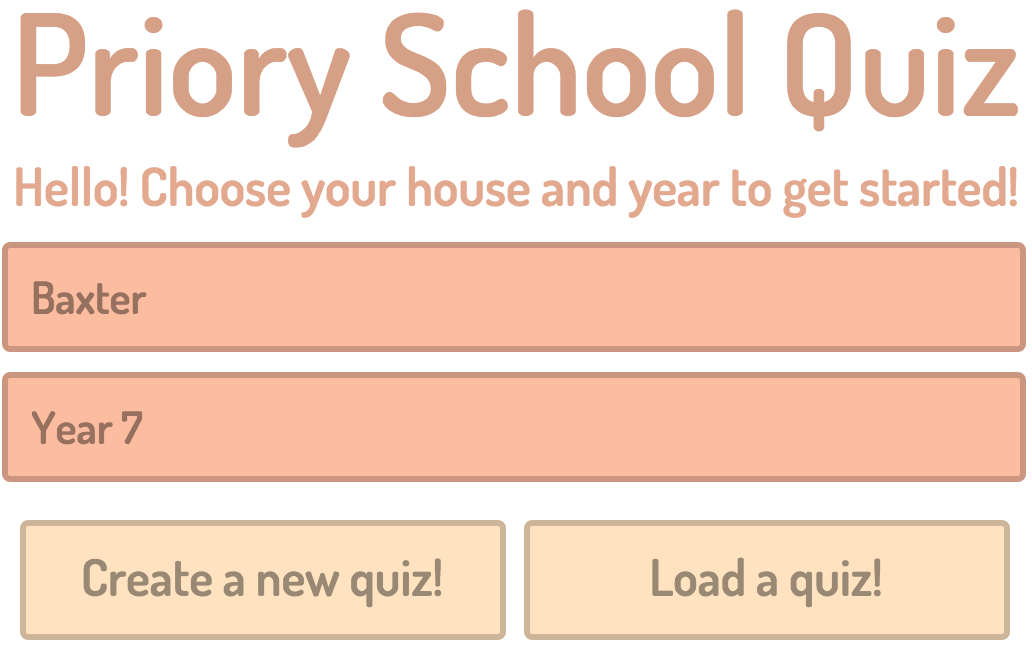
\includegraphics[scale=0.35]{testing/colours/baxter}
  \caption{Test outcome for Baxter's colours.}
\end{figure}

\begin{figure}[!htbp]
  \centering
  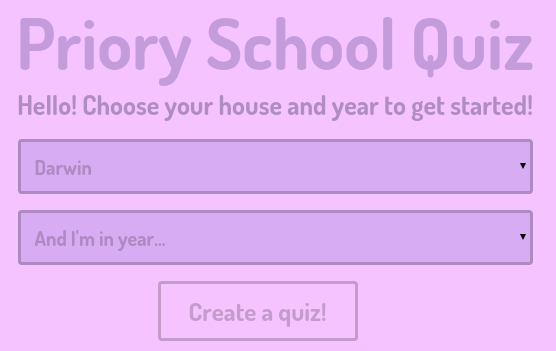
\includegraphics[scale=0.35]{testing/colours/darwin}
  \caption{Test outcome for Darwin's colours.}
\end{figure}

\begin{figure}[!htbp]
  \centering
  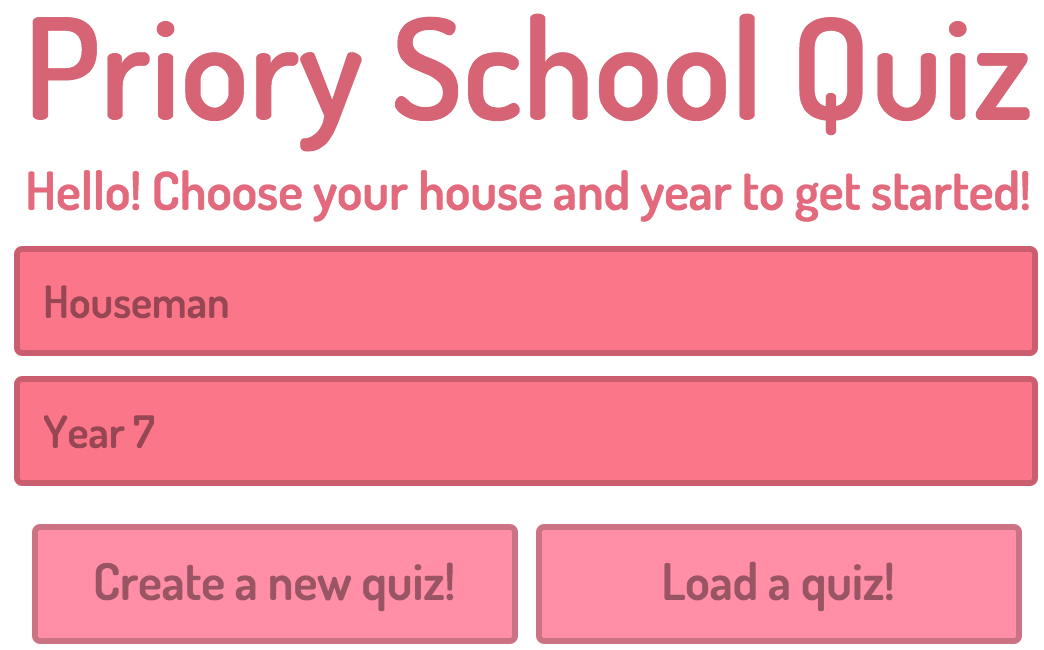
\includegraphics[scale=0.35]{testing/colours/houseman}
  \caption{Test outcome for Houseman's colours.}
\end{figure}

\begin{figure}[!htbp]
  \centering
  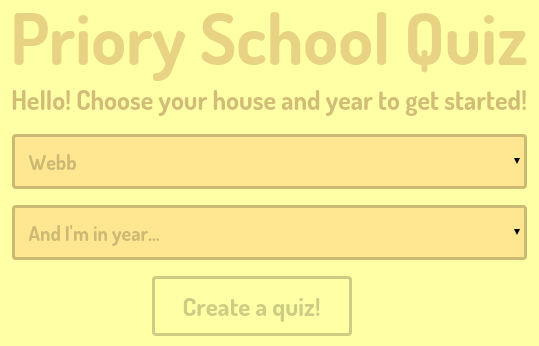
\includegraphics[scale=0.35]{testing/colours/webb}
  \caption{Test outcome for Webb's colours.}
\end{figure}

% subsection colour_tests (end)
